\documentclass{jsarticle}

\usepackage[dvipdfmx]{graphicx}

\title{Flutterであなたもアプリデベロッパー!!}
\author{}
\date{}

\begin{document}
    \maketitle
    \tableofcontents

    \section*{はじめに}
        この文章は、筆者が最近アプリ開発を久しぶりにかじり出したら楽しくなっちゃった結果生み出された駄文です。
        心してお読みください。

        この文章を通じて、Flutterというフレームワーク\footnote{システム開発を簡単にできるように用意されたプログラム}
        を使用して基礎的なアプリ開発ができるようになることを目標としています。想定している読者は以下の通りです。

        \begin{itemize}
            \item アプリ開発をしたことないけどしてみたい人。
            \item XcodeやAndroid Studioを使ったアプリ開発はめんどくさい人。
            \item 暇な人。
        \end{itemize}

        逆に、今までアプリ開発をいろいろやってきて、「新しいフレームワークでも調べながら
        ごりごりいじれるよ!」みたいな人は想定していません。お帰りください。

        この文章では、基本的な専門用語も脚注などで軽い説明を入れてあるつもりです。
        わからないところが出てきても、とりあえず少し先まで読んでみてから調べることをお勧めします。

        また、本書で使用しているコードは筆者のGitHub(https://github.com/50m-regent/magazine)で
        全て公開しているので、ぜひ参考にしてください。

        最後に、本書に関してご意見などありましたら筆者のTwitter(@50m\_regent)までご意見を
        いただければ幸いです。

        では、Flutterの世界に飛び込みましょう!

    \section*{Flutterって何?}
        皆さんはGoogleという会社を知っているでしょうか。
        むしろ知らない人がいるのかというレベルですね。
        言わずと知れた世界の大企業です。
        そんなGoogleが開発しているWeb・アプリ開発ようフレームワークがFlutterです。
        皆さんが普段使っているようなGoogleのアプリも、このフレームワークを使用して実装されています。

        さて、そんなFlutterですが、DartというこれまたGoogleが開発している言語を使用してソースを書きます。
        個人的に他のアプリ開発方法\footnote{Xcodeを使用したiOSアプリ開発や、Android Studioを使用した
        Androidアプリ開発}と比べて嬉しいなと感じた点を挙げてみます。

        \begin{itemize}
            \item GUI\footnote{マウスを使って直感的な操作をできる画面}で設定やアプリの構成をする必要がなく、
                 コーディングで全て行うので、シンプルな開発ができる。
            \item iOS、Android両対応のアプリを簡単に作ることができる。
            \item 標準でデザインに使えるような部品が用意されている。
        \end{itemize}

        Flutterにはまだまだ沢山の長所がありますが、逆に欠点もあります。
        中でも最大のものは、日本語の解説が少ないという点です。
        筆者が開発してる時は、8割以上海外のウェブページを参考にしていました。
        
        これからFlutterに触れる人たちが英語によって門前払いを食らわずに、
        この文書を通して少しても忌避感をなくせれば幸いです。

    \section*{環境構築}
        さて、まずはじめにFlutterで開発ができる環境を作らないといけません。

        Android StudioというIDE\footnote{統合開発環境。一つのソフトウェアでシステム開発ができるようにしてあるもの}
        を使用する方法と、VScodeというエディタ\footnote{テキストファイルを編集するソフト}を使用する方法
        がありますが、個人的にオススメのVScodeの方を解説していきたいと思います。
        「Android Studioで開発しないと耐えられない!」という人は各自調べてください。

        なお、iOSアプリの開発をするにはOS Xが必須です。ご了承ください。

        \subsection*{全OS共通編}
            \subsubsection*{SDK\footnote{ソフトウェアを使うためにセットにしてあるファイル}のダウンロード}
                まず始めに、PCがFlutterを認識できるようにします。
            \begin{enumerate}
                \item Flutter公式サイト(https://flutter.dev/)にアクセス。
                \item 図\ref{fig:flutter_main_page}の"Get Started"を押した後、
                      図\ref{fig:flutter_download_page}のページで適当なOSを選択。
                \item flutter\_\{OS名\}\_vX.X.X-stable.zipをダウンロード。
            \end{enumerate}

            \begin{figure}[ht]
                \centering
                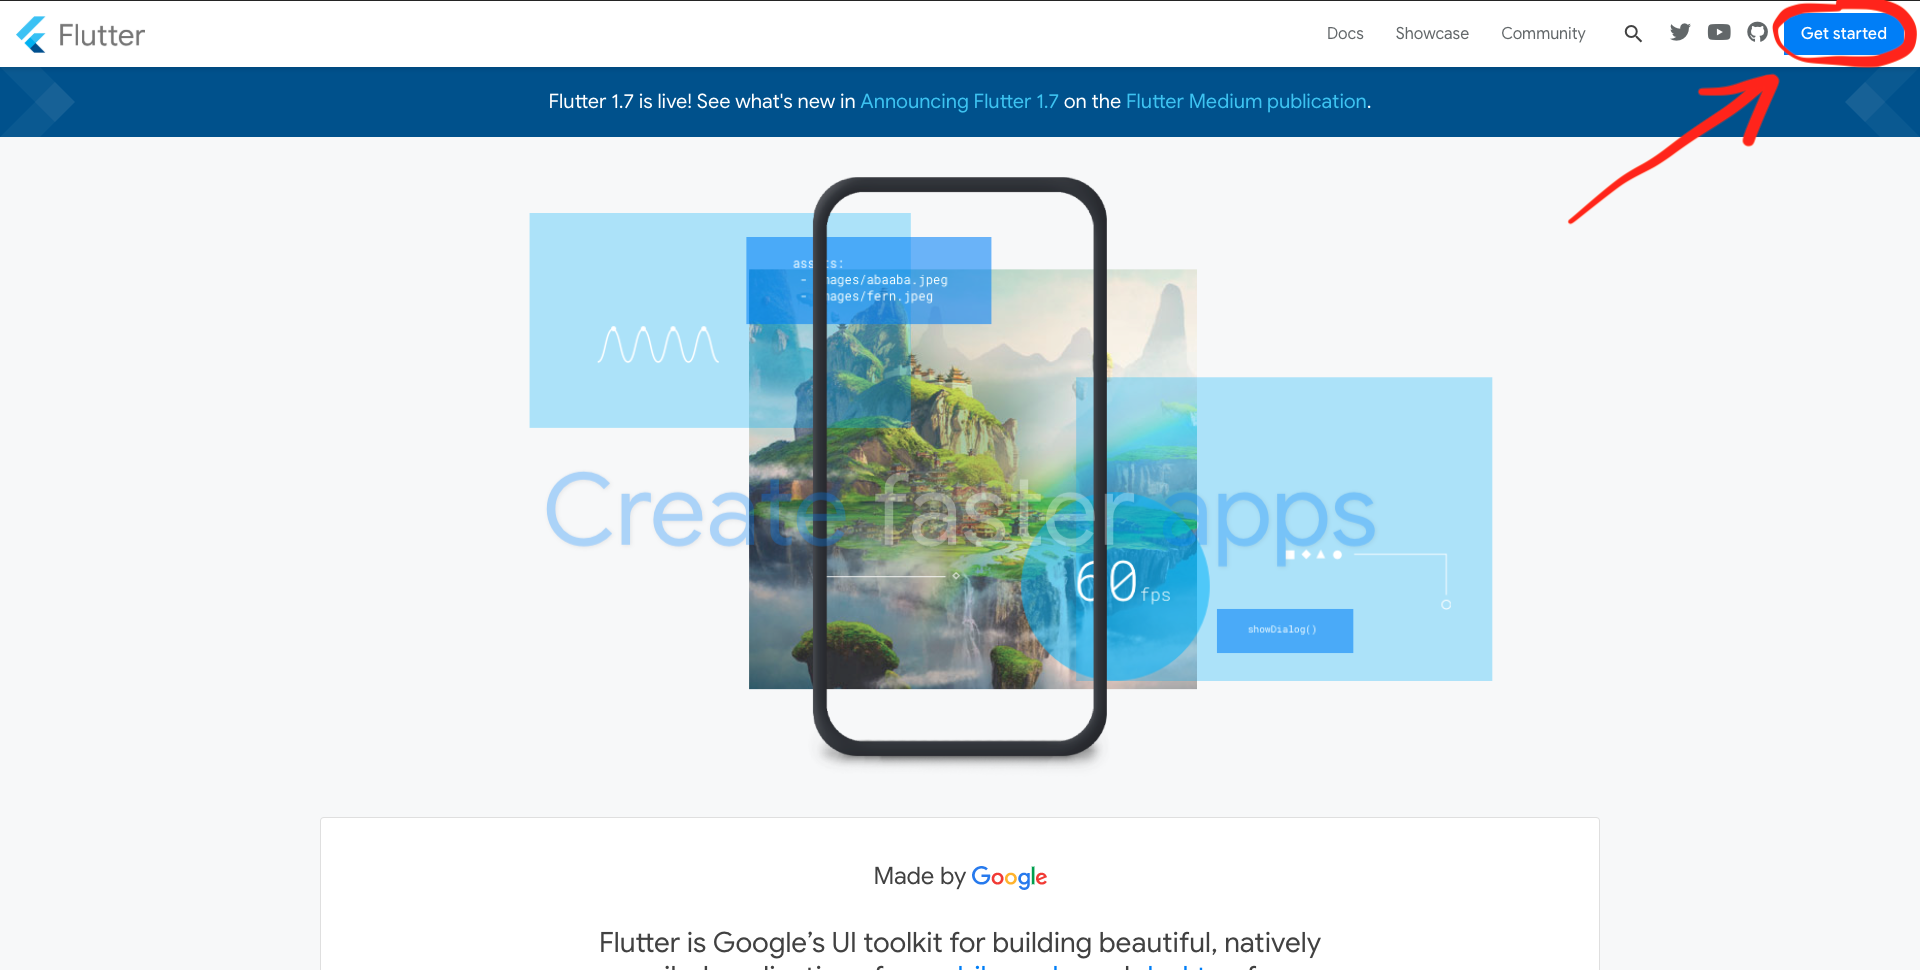
\includegraphics[width=10cm]{images/flutter_main_page.png}
                \caption{Flutter公式ページ}
                \label{fig:flutter_main_page}

                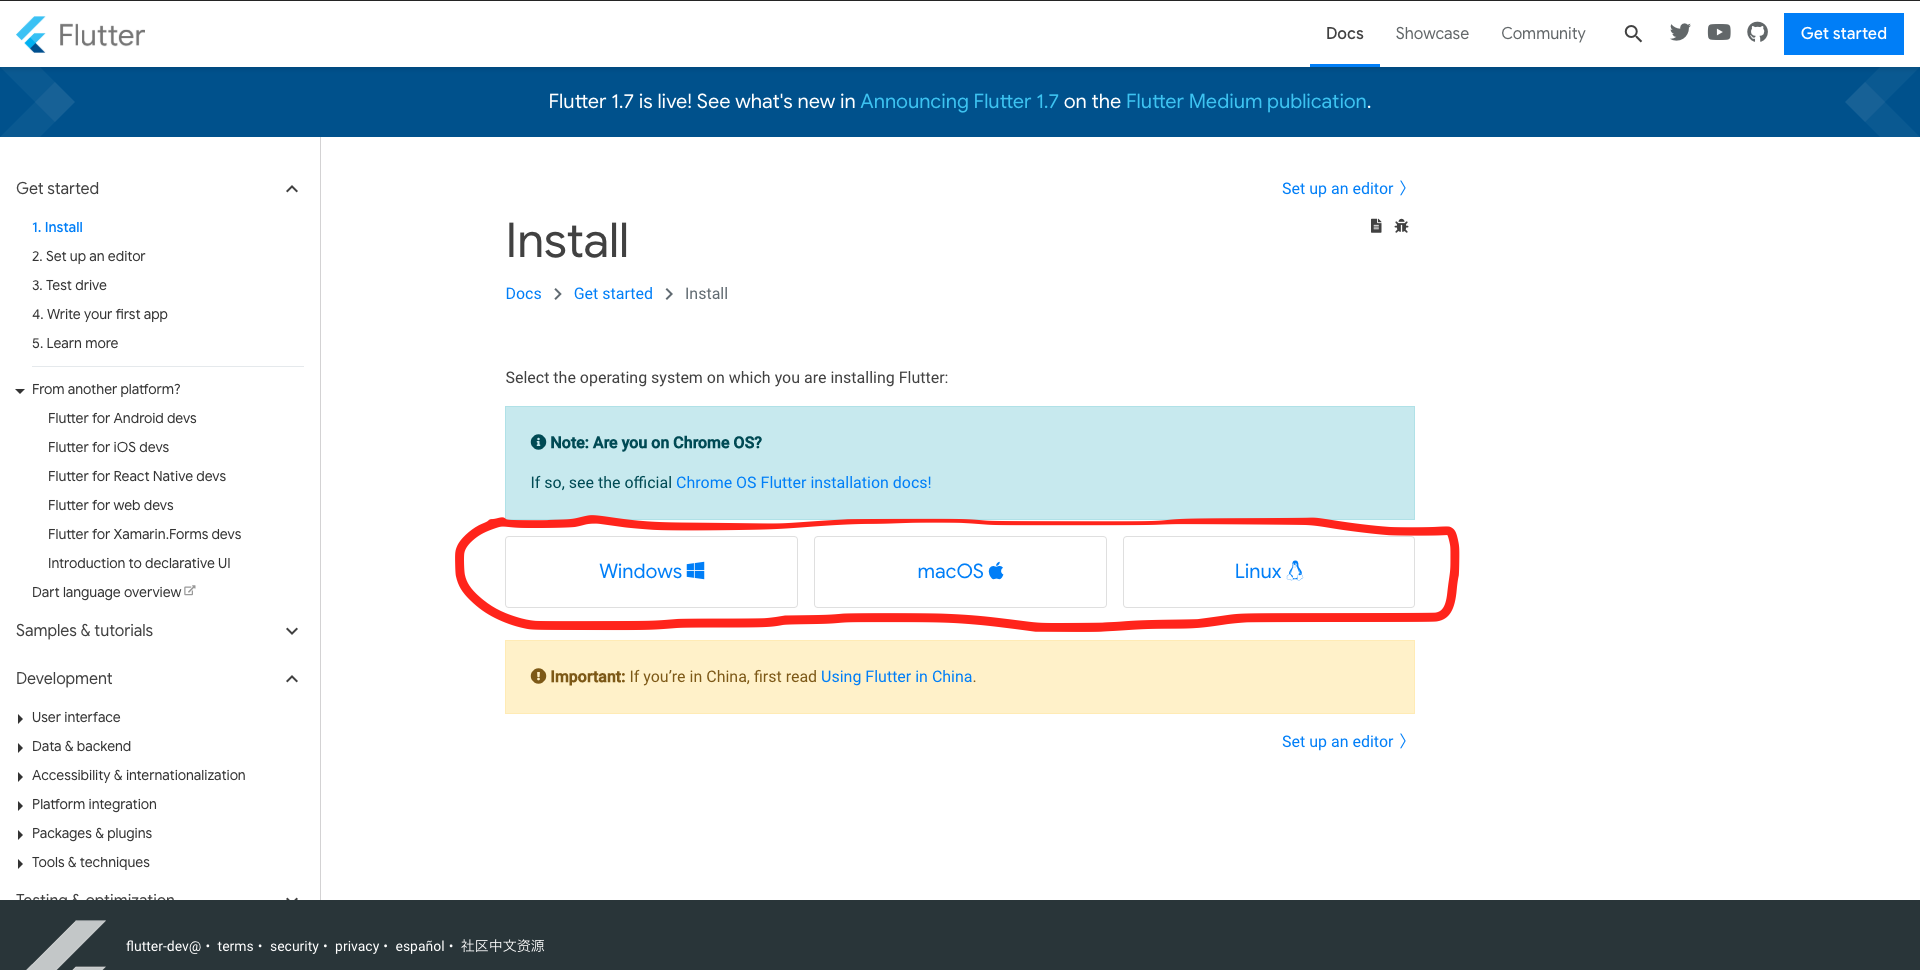
\includegraphics[width=10cm]{images/flutter_download_page.png}
                \caption{Flutterダウンロードページ}
                \label{fig:flutter_download_page}

                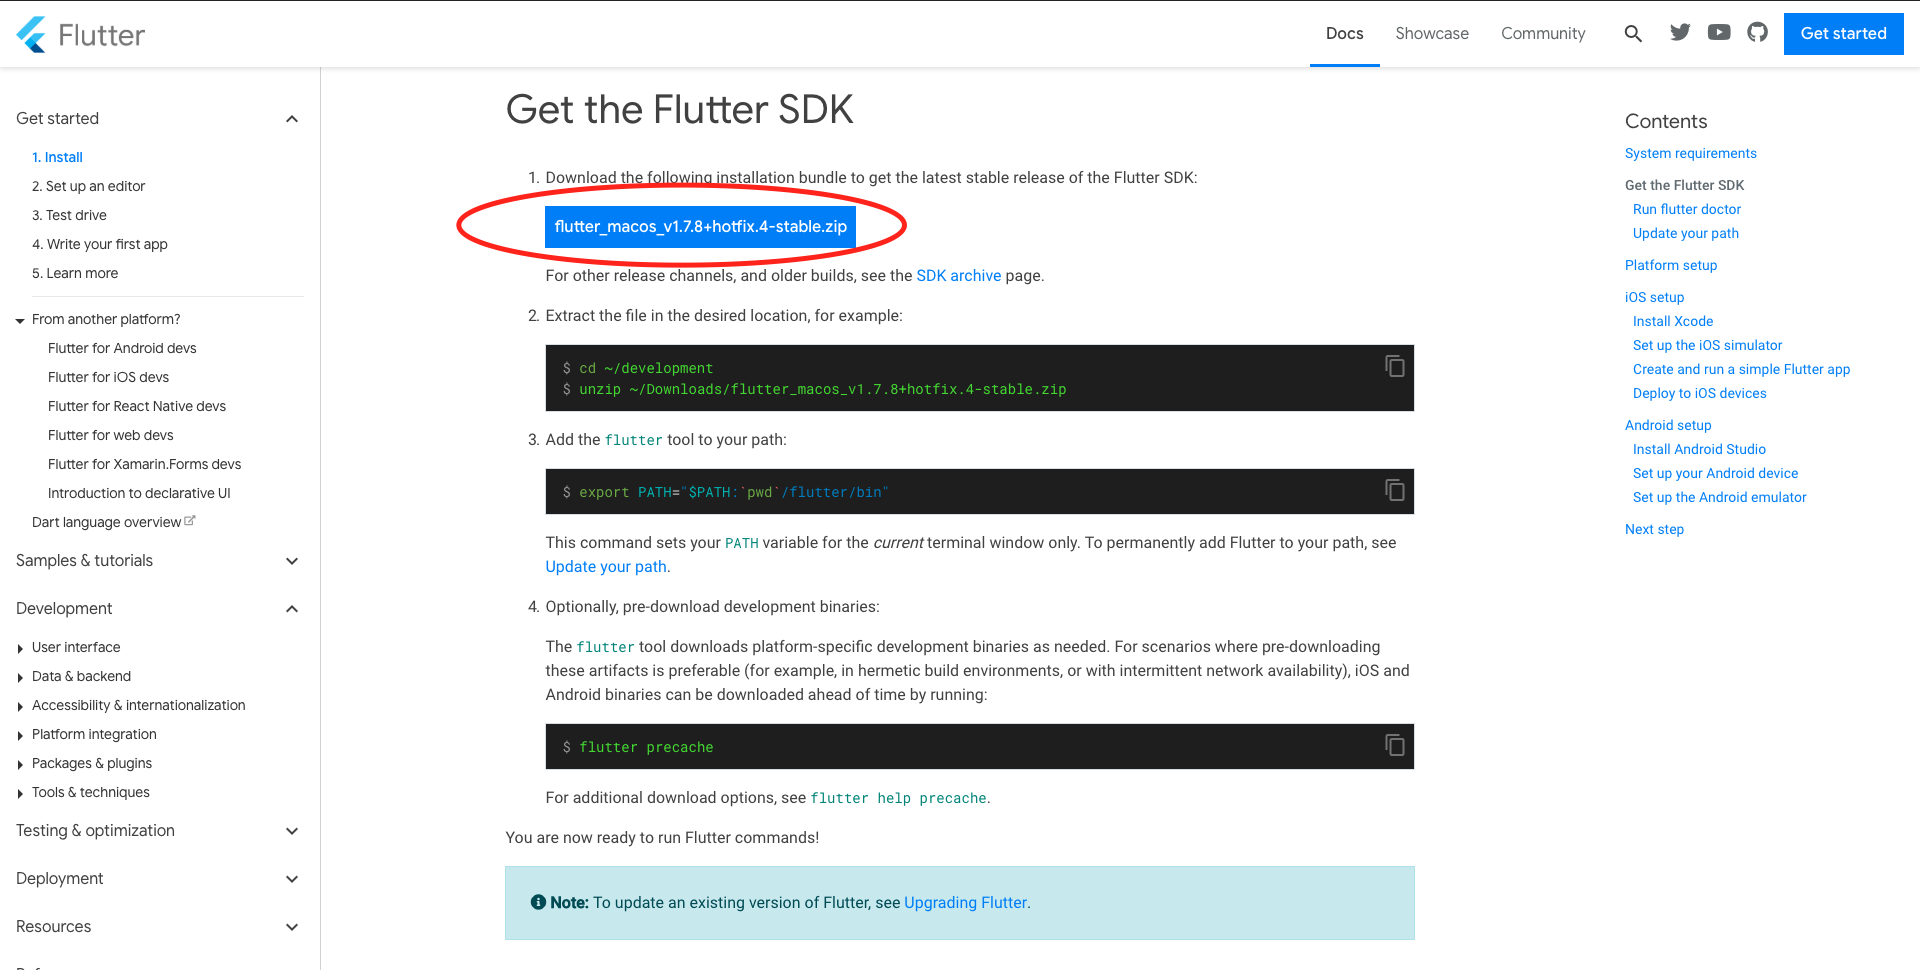
\includegraphics[width=10cm]{images/flutter_download_link.png}
                \caption{Flutterダウンロードリンク}
                \label{fig:flutter_download_link}
            \end{figure}

        \subsection*{Windows編}
            さて、ここからはWindowsとOS X、Linuxで手順が変わってくるので、この説では
            Windowsに重きを置いて残りの解説をします。

            \subsubsection*{SDKのインストール}
                共通編でダウンロードしてきたSDKをPCにインストールしましょう。

                \begin{enumerate}
                    \item 任意の場所\footnote{任意の場所がよくわからない人はデスクトップとかが安心です}
                          にダウンロードしてきたzipファイルを解凍。
                    \item 解凍したフォルダ内のflutter\_console.batを実行。
                \end{enumerate}

                Flutterコンソールが立ち上がれば成功です!

                また、Flutterコンソールではなく、普段使っているコンソールでFlutterをいじりたい方は、
                「Flutter パス設定\footnote{OSがプログラムを認識できるようにプログラムの場所を示すこと}」
                などで検索してみたください。

            \subsubsection*{Android Studio、VScodeのインストール、設定}
                
            
\end{document}